\documentclass{standalone}

\usepackage{tikz}
\usetikzlibrary{arrows,decorations.pathmorphing,positioning,fit,petri}
\usetikzlibrary{calc,intersections,through,backgrounds,graphs}
\usetikzlibrary{patterns,decorations.pathreplacing}

\begin{document}

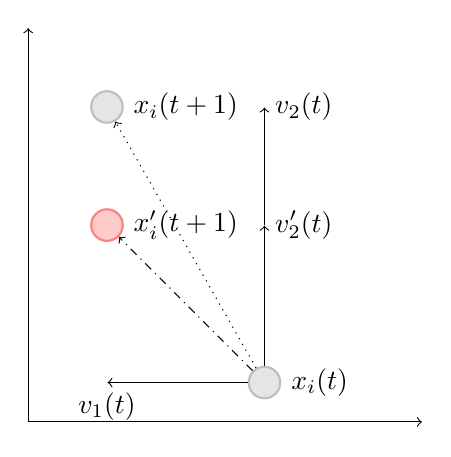
\begin{tikzpicture}
	% Styles
	[
	point/.style={circle,inner sep=0pt,minimum size=0mm},
	vpoint/.style={circle,draw=gray!50,fill=gray!20,thick, inner sep=0pt,minimum size=4mm},
	endpoint/.style={circle,draw=red!50,fill=red!20,thick, inner sep=0pt,minimum size=4mm},
	]
                      
	% Axis
	\draw[->] (0,0) -- (5,0);
  	\draw[->] (0,0) -- (0,5);

	% Nodes
	\node at (3,0.5)	(xi1)	[vpoint]	{};
	\node at (1,4)	(xi2) [vpoint] {};
	\node at (1,2.5)	(xi3) [endpoint] {};
	\node at (3,2.5) 	(v2) [point] {};
	\node at (3,4)	(v22) [point] {};
	\node at (1,0.5)	(v1) [point] {};

	% Arrows	
	\draw[->] (xi1) -- (v2);
	\draw[->] (v2) -- (v22);
	\draw[->] (xi1) -- (v1);
	\draw[->,dotted] (xi1) -- (xi2);
	\draw[->,dashdotted] (xi1) -- (xi3);

	% Text
	\node at (3.7,0.5) {$x_i(t)$};
	\node at (2,4) {$x_i(t+1)$};
	\node at (2,2.5) {$x_i'(t+1)$};
	\node at (3.5,4) {$v_2(t)$};
	\node at (3.5,2.5) {$v_2'(t)$};
	\node at (1,0.2) {$v_1(t)$};
\end{tikzpicture}

\end{document}